\documentclass[tikz]{standalone}

\usepackage{tikz}
\usetikzlibrary{positioning}

\begin{document}

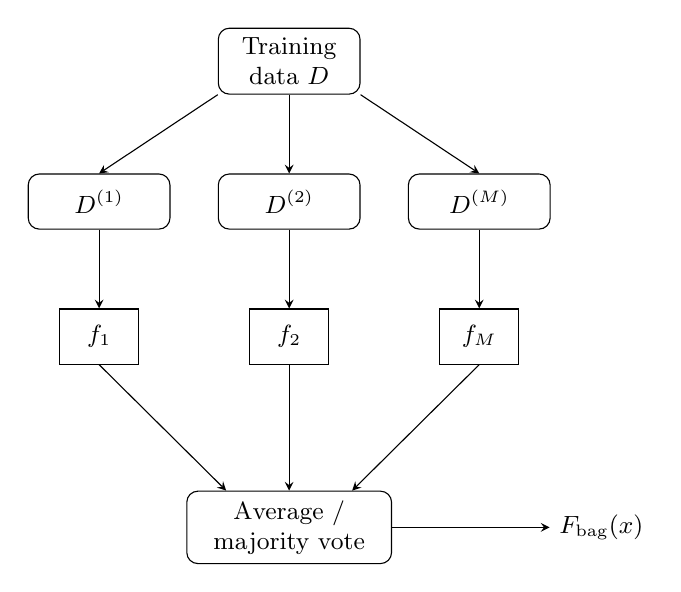
\begin{tikzpicture}[
    >=stealth,
    every node/.style={font=\small},
    box/.style={draw,rounded corners,minimum width=18mm,minimum height=7mm,align=center},
    tree/.style={draw,rectangle,minimum width=10mm,minimum height=7mm,align=center}
]

% Original dataset
\node[box] (data) {Training\\data $D$};

% Bootstrap samples
\node[box,below left=10mm and 6mm of data]  (b1) {$D^{(1)}$};
\node[box,below       =10mm of data]        (b2) {$D^{(2)}$};
\node[box,below right=10mm and 6mm of data] (b3) {$D^{(M)}$};

% Arrows from original data to bootstraps
\draw[->] (data.south west) -- (b1.north);
\draw[->] (data.south)      -- (b2.north);
\draw[->] (data.south east) -- (b3.north);

% Base learners (trees)
\node[tree,below=10mm of b1] (t1) {$f_1$};
\node[tree,below=10mm of b2] (t2) {$f_2$};
\node[tree,below=10mm of b3] (t3) {$f_M$};

\draw[->] (b1) -- (t1);
\draw[->] (b2) -- (t2);
\draw[->] (b3) -- (t3);

% Aggregation box
\node[box,below=16mm of t2,minimum width=26mm] (agg) {Average /\\majority vote};

\draw[->] (t1.south) -- ([xshift=-8mm]agg.north);
\draw[->] (t2.south) -- (agg.north);
\draw[->] (t3.south) -- ([xshift=8mm]agg.north);

% Output
\node[right=20mm of agg] (out) {$F_{\mathrm{bag}}(x)$};
\draw[->] (agg.east) -- (out.west);

\end{tikzpicture}

\end{document}

